The recertification process is triggered when specific security conditions are met after a system undergoes a configuration change; the components of such process need to adapt to the new approach, and for the current step this thesis is taking, their models inevitably need to change. Therefore, this chapter introduces all the required components: i) attributes, ii) properties, iii) trigger, and iv) tests and evidence collection models. In addition, the scoring system guides the certification process, allowing one to express how strong the certificate should be. Moreover, properties and attributes are still at the basis of the proposed certification scheme, but properties are now referred to as micro-properties, each of whom is categorized under a specific macro-property; such separation grants a wider grade of control over the scoring system. Furthermore, the trigger is a new component whose task is to send an alert whenever a configuration change alters one or more security properties, detailing all the needed information about such properties and the involved attributes. Finally, the evidence collection model is built around the other components' models and allows specifying detailed information about the testing phase that must be executed. The interaction between such components and the general flow of the proposed process is shown in figure \ref{fig:comps}.

Given the above overview of the main components of the proposed certification scheme, it is useful to keep in mind a simple example scenario that will support the further explanation of the components in the following sections.

\begin{figure}[ht]
    \centering
    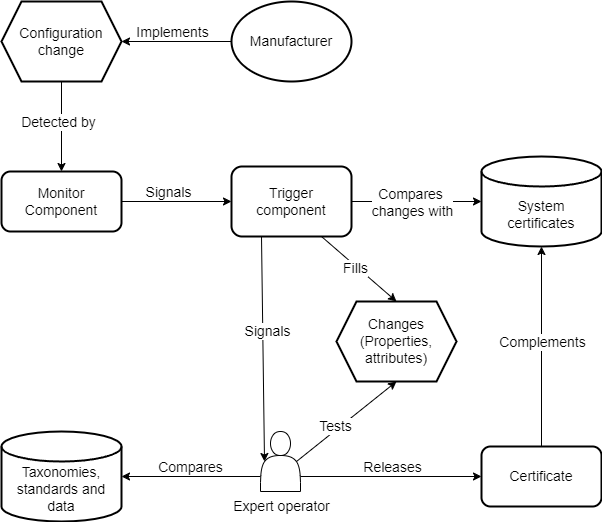
\includegraphics[scale=0.7]{images/components.png}
    \caption{Proposed scheme's components and interactions}
    \label{fig:comps}
\end{figure}


\section{A Simple Example Scenario}
\label{scenario}
This section illustrates a simple contextual example to improve the visualization the proposed idea; we note that many details of this example are further developed in the following sections. This example scenario shows how a specific situation could be handled using the proposed scheme and will be used as a reference in the next sections:

Let us consider a smart city environment where the manufacturer needs to add security cameras. Since the contract with the system's owner requires a certificate of proof that any produced data is secured, the system needs a quick re-validation to prove that the recorded images are indeed securely stored. This scenario could involve many properties, however, only two of them and one attribute for each property will be considered in this example for simplicity: referring to the properties taxonomy in appendix \ref{taxonomy}, let us consider the secure storage paragraph, which includes the following properties and attributes:

\begin{enumerate}
    \item The ability to support data encryption at rest (encrypt passwords, device id and other authentication data) and the considered attribute is the following: given that the encryption algorithm is the AES \cite{daemen1999aes}, the attribute's value can be i) 128 bits, ii) 192 bits, or iii) 256 bits.
    
    \item The ability to "sanitize" or "purge" specific or all data in the device and the considered attribute is the followingn: given that the storage eraser algorithm is the U.S. Department of Defense (DoD) 5220.22-M algorithm \cite{fischer2017dod}, an attribute can be the number of times the data is overwritten, and the value can be 3 or 7.
\end{enumerate}





\section{The scoring system}
Before introducing the main components of the certification scheme, it is important to present the concept of score and how the scoring system works; a score is assigned to each attribute based on its value and the purpose and context of the entire system. The score of a property is then calculated by summing the scores of its attributes. Finally, the weighted sum of all the properties scores determines the certificate's strength; additionally, for the certificate to be valid, such a total must reach a pre-determined threshold. Expert manual operators should decide the score values and the thresholds with the help of taxonomies, standards and knowledge.

\begin{example}
\label{xmp:1}
Following the example scenario in section \ref{scenario}, the ranges of scores assigned to the attributes could be [10, \dots, 70] for the AES algorithm attribute and [40, \dots, 80] for the U.S. DoD 5220.22-M algorithm.
Since the sum of the properties scores finally defines the certificate's strength, such a sum must reach at least the defined threshold, which could be set at 100 with a weight of 1, for example.
\end{example}


\section{Attributes}
As for the state-of-the-art approaches, properties will still be modelled using attributes that define them at a lower level; more specifically, in the proposed approach, attributes define micro-properties, and are defined in a slightly different way from state-of-the-art schemes. 

\begin{defn}
An attribute \(a\) is defined as a pair \((\hat{a}, [value_{min}, value_{max}])\) where \(\hat{a}\) is the abstract attribute and \(value_{i}\) is a possible value of \(a\). 
\end{defn}

In other words, an attribute is now defined by its name and the list of values it can assume. We note that the range of possible values is considered sorted by relevance, from the less relevant to the most relevant. For example, the value of the response time of a device is more relevant the lower it is; contrary, the value of a storage size is more relevant the bigger it is.

The score range of an attribute should be decided by an expert person having knowledge of the system and the context; such range should be balanced, setting the lowest score corresponding to the lowest relevant valid value and vice-versa.
The linear mapping (mapping that maintains a constant ratio between points) operation in the equation \ref{eqn:mapping} allows mapping values between two ranges, in this case, values and scores.

\begin{equation}
\label{eqn:mapping}
    q = \left \{ (p - A) \times \frac{D - C}{B - A} + C \bigm| [A, B] \in \mathbb{N} \wedge [C, D] \in \mathbb{N}  \right \}
\end{equation}

Considering the range of valid attribute values from A to B, the range of scores from C to D, and the actual attribute value p, the mapping allows computation of the corresponding score value q.
A linear mapping requires two operations: a scaling operation to make the ranges the same size and an offset operation to align the ranges. Since scaling is always relative to the origin, the first step is to shift the range [A, B] to the origin by subtracting A from p; next, scale p by the ratio of the range sizes (D-C)/(B-A). Finally, shift this value to the start of the [C, D] range by adding C, resulting in the equation \ref{eqn:mapping}. By rearranging the terms of the equation, it is possible to extract the scale and offset factors that compose it:

\[scale = \frac{D - C }{B - A}\]
\[offset = -A \times \frac{D - C}{B - A} + C\]
\[q = \left ( p \times scale \right ) + offset\]


This equation maps the attribute's values range to the scores range spreading the values evenly (e.g., “equal importance” expressed with W[0] = 1/n, W[1] = 1/n, \dots , W[n]= 1/n). If the attribute's values are not numerical, they should be pre-emptively mapped to a list of indices; the indices list should then be used instead of the attribute's values; finally, the result should be rounded up in case it does not exactly match a value because rounding down would result in a weaker-than-expected certificate. For example, for the micro-property Interface Control (ref), it is necessary to have a list of supported communication technologies that could include IEEE 802.11, Bluetooth and Ethernet connections; such a list might be mapped with an index list [1,2,3] where each index represents one of the elements.

\begin{example}
Following Example \ref{xmp:1}, equation \ref{eqn:mapping} can be used to determine which values will be tested for each attribute. First, a couple of steps need to be done: i) substitute the lists of values with lists of indices; [1,2,3] for the AES algorithm attribute (\(q_1\)) and [1,2] for the U.S. DoD 5220.22-M algorithm attribute (\(q_2\)), and ii) the threshold of 100 should be evenly distributed across the score ranges to determine the score each attribute should obtain, namely, T/n where T is the threshold (100) and n is the total number of attributes (2). Then, the values can be discovered using the equation:
\begin{align*}
  q_1 = (50 - 10) \times \frac{3 - 1}{70 - 10} + 1\\
  q_1 = 40 \times \frac{2}{60} + 1 \\
  \llap{$\rightarrow$\hspace{50pt}} q_1 = \Bigl\lceil\frac{7}{3}\Bigr\rceil = 3
\end{align*}
\begin{align*}
  q_2 = (50 - 40) \times \frac{2 - 1}{80 - 40} + 1\\
  q_2 = 10 \times \frac{1}{40} + 1 \\
  \llap{$\rightarrow$\hspace{50pt}} q_2 = \Bigl\lceil\frac{5}{4}\Bigr\rceil = 2
\end{align*}

When translating back the indices to the real values, the results show that to reach at least the set threshold of 100, attribute \(q_1\) needs to have a value of 256 bits and attribute \(q_2\) needs to have a value of 7.
\end{example}

The mapping also allows the system to compute the minimum values that each attribute of each micro-property needs to have to release a certificate with the minimum effort. Such values should then be gathered with a simple getter function.

\[ComputeMinValues([a_1, \dots , a_n], threshold)\]
\[GetMinValue(aj) \rightarrow {value_a}_j\]

\section{Properties}
The old properties are now referred to as micro-properties, and they have been organized into three categories referred to as macro-properties.
\begin{defn}
A micro-property p is a pair \(\left (\hat{p}, \left \{  (a_1, value_1), \dots , (a_n, value_n)\right \} \right )\) 
where \(\hat{p}\) is the abstract micro-property and \(\left ( a_i ,value_i \right )\) is a pair representing an attribute of the property and its value.
\end{defn}

In other words, micro-properties are defined by their attributes and the corresponding values.


On the other hand, macro-properties are intended to regroup micro-properties that influence similar aspects of the system; more specifically, every micro-property contributes to one of the macro-properties, namely, \textit{Confidentiality}, \textit{Integrity} and \textit{Availability}. Macro-properties have a specific function in the proposed approach, helping with the micro-properties score attribution; since the thresholds will be based on the macro-properties, every micro-property's score will influence its macro-property final weighted score.

\begin{defn}
A macro-property of the system P is defined as a triple \\ \( \left ( \hat{P}, \left \{(p_1, score), \dots , (p_n, score )\right \}, wscore \right ) \) where \(\hat{P}\) is the abstract macro-property, \( \left (p_i, score \right ) \) is a pair representing a micro-property and its score, and \textit{wscore} is the total weighted score of the macro-property; the weight determining the final result should depend on the context.
\end{defn}

By way of explanation, macro-properties act as abstract containers of micro-properties and scores, allowing for better control over which categories of micro-properties should be prioritized during a certification process.

\begin{example}
Following the example in Section \ref{scenario}, the properties described translate directly into micro-properties, which are then categorized under the Confidentiality macro-property; the threshold set also refers to the same macro-property.
\end{example}

\section{Trigger}
\label{trigger}
The trigger is a component detecting security changes in the system, evaluating them and acting in case these changes should impact crucial security properties. The trigger should also have continuous access to the system's information and certificates to detect changes accurately. The framework should access such changes through the \textit{Changes} function. 

\begin{defn}
The \textit{Changes} function is defined as \(Changes() \rightarrow \left \{ \left ( p_j, \left \{ a_k \right \} \right ) \right \} \), where \(p_j\) is a micro-property of the system and \( \left \{a_k \right \} \) is the set of specific attributes impacted by the update.
\end{defn}

Such a function includes multiple background operations that the system has to deal with; these functionalities should probably include a monitoring framework for change detection. The monitoring should be invoked automatically every time a system (or context) update occurs. It should then compare the updated changes with the security properties and their attributes; any change over a security property should be immediately added to the \textit{Changes} function output list. Moreover, the trigger component should also be notified about the availability of new changes.


\section{Evidence Collection Model}

Evidence collection is the process that, given a system and a property, gathers evidence proving the system holds such property through a series of tests.

\begin{defn}
    A test \textit{t} is now modelled as a tuple \( \left ( \hat{p}, \left (a_j, value_j, c_j, \left \{ cnd_k \right \} \right ) \right ) \) where
    \begin{itemize}
        \item \( \hat{p} \) is the micro-property to test;
        \item \(a_j\) is an attribute of the micro-property;
        \item \(value_j\) is the expected value of the attribute;
        \item \(c_j\) is the code to execute to gather evidence over the attribute \(a_j\);
        \item \( \left \{ cndk \right \} \) is the set of conditions that need to be satisfied by the test execution.
    \end{itemize}
\end{defn}

In other words, each test case is specifically aimed at demonstrating that a system's attribute holds for a specific value; once all the attributes included by a micro-property have been demonstrated, the micro-property can also be considered demonstrated.
Additionally, the evidence collection model allows having a more defined structure over
which evidence can be gathered.

\begin{defn}
The evidence collection model \(\mathcal{E}\) is defined as a set of elements, one for each micro-property, and it is modelled as \(  \left \{ \left \{ t_j \right \} {_{\hat{p}_i}} \right \} {_{\hat{P}_j}} \) where \( \hat{P}_j \) is a macro-property, \( \hat{p}_i \) is a micro-property, and \(t_j\) is the test to evaluate the attribute \textit{j} (\(a_j\)).
\end{defn}

In other words, the evidence collection model E is a list of test cases where each test aims at verifying that an attribute holds a specific value. The gathered evidence is then eventually stored in the released certificate.

\section{Certification Model Definition}
Once the trigger component starts the process by providing the system changes information, an important component that needs to be used for the recertification is the set of old certificates \(\mathcal{C}\); they contain all the demonstrated properties with their score and collected evidence prior to the update. Therefore, the proposed scheme is expected to provide a function \textit{Ephemeral} to obtain the certification model for the updated system.

\begin{defn}
The \textit{Ephemeral} function is defined as \(Ephemeral(\mathcal{C}, system_{t+1}) \rightarrow {\mathcal{M}}_{t+1} \), where 
\(\mathcal{C}\) is the set of certificates released for the system up to the time \textit{t}, \textit{t+1} represents the time after the update, and \(\mathcal{M}_{t+1}\) is the certification model for the updated system.
\end{defn}

Once the new certification model is computed, it will be possible to call the \textit{Execute} function that will execute the tests on the system based on the given certification model returning the new certificate if all the requirements are satisfied. 

\begin{defn}
The certification model is defined as 
\(\mathcal{M} = \left ( \left ( P_1, P_2, P_3 \right ), \mathcal{E} \right )\) where \(P_i\) is a macro-property and \( \mathcal{E} \) is the evidence collection model.
\end{defn}
Namely, the macro-properties that compose the certification model \(\mathcal{M}\) are:
\begin{itemize}
    \item \(P_1\) is the Confidentiality macro-property
    \item \(P_2\) is the Integrity macro-property
    \item \(P_3\) is the Availability macro-property
\end{itemize}
 
The framework should then be able to call the \textit{Execute} function using the certification model to deliver a new ephemeral certificate.


\begin{defn}
The \textit{Execute} function is defined as \( Execute(\mathcal{M}_{t+1}) \rightarrow \mathcal{C} \cup \{c_{t+1}\} \), where \( \mathcal{C} = {c_0, \dots , c_t} \) and \(c_i\) is the certificate released at time \(i\).
\end{defn}
 The execute function allows obtaining the new certificate for the updated system and automatically adds it to the set of system's certificates \(\mathcal{C}\).
 
 \begin{defn}
 Each certificate is then defined as a set of pairs \( (p, \{e_j\}) \), where \(p\) is a micro-property with the set of evidences supporting it \( (\{e_j\}) \).
 \end{defn}
 
 The system will finally be attributed a new certificate that will complement all the previously obtained ones and will carry all the information of the re-certification process that occurred after the update, including tested micro-properties and attributes, tests information and gathered evidence.



\section{Assumptions}

For the next chapters, it is essential to clarify all  the major assumptions made during the design phase of the proposed certification process. As described in chapter \ref{cap2}, the current efforts in the IoT world are directed toward highly distributed systems (Edge computing) that involve some central computing nodes (Cloud computing). Therefore, when referring to IoT systems in the next chapters, it will be implied that the system will be composed of a Cloud layer, an Edge layer and an IoT layer. We note that the ToC model defined in chapter \ref{cap2} is still valid and has not been considered in this thesis work for simplicity, although in future, it could be modelled differently to better suit the new frameworks. Furthermore, it should be noted that this thesis' focus is on maintaining the certification's validity during the system's life cycle, mainly after some configuration change. Hence, when dealing with examples in the future chapters, it will be assumed that every system has already been fully certified with a standard certification model (e.g. Common Criteria) at the start of its functions. The proposed re-certification process should be aware of a threshold indicating the number of changes a system has to go through before the process is triggered. Such a threshold should be preemptively tested and precisely studied, possibly in the manual certification process, as it depends entirely on the context. It will be assumed that this value is known and irrelevant in future examples. There is also a major assumption in current standards that needs to be removed to apply the proposed solution; such assumption is to know a priori all the properties, attributes and mechanisms of the system. Only a part needs to be known; the rest should be found or inferred in some non-intrusive and lightweight manner. The risk with such an assumption is to debilitate the chain of trust and reduce the quality of the certification; if an attribute is discovered to have an invalid value, the entire certificate might be invalidated..
A couple of assumptions need to be made regarding the proposed certification model. Specifically, the trigger component is assumed to have access to the system's information, such as the old certificates; it is also assumed that the trigger has the capabilities to compute the system's changes over properties and their attributes. Another important point is the assumption of having an expert person knowing how to precisely balance the score values over the attributes given the knowledge of the system and the environment where it is deployed.






\section{Ephemeral Certification Process}
Chapter \ref{cap2} shows that previous iterations of certification frameworks dealt with non-functional properties, attributes and mechanisms, assuming to know them when needed. This approach was valid in Cloud environments because all the required properties to be certified were manually pre-established and specified during a preparation phase before the certification execution. However, the process implied a rather large overhead when certifying a whole new system or issuing a recertification process after a small configuration change. In Cloud environments, a slow process is acceptable due to the small number of changes a Cloud system usually has to go through and the high accuracy requirements. On the other hand, IoT environments are highly dynamic, unique and continuously subject to small configuration and patch changes making this approach no longer feasible due to the high overhead each certification process would introduce and the resource cost, especially in the manual preparation phase.

As described in chapter \ref{cap2}, a certification process is usually made of four main steps: i) definition of the non-functional properties ii) definition of the certification target and of the mechanisms that will allow testing a given property iii) tests definition, aimed at collecting evidence proving the property iv) tests execution and evidence collection. So, for example, a test to collect evidence over the attribute \(x\) would be a pair \( (M_x, (c, R_e) ) \) where \(M_x\) is the mechanism the system offers to test the attribute \(x\), c is the code to execute, and \(R_e\) is the expected result of the test code execution; if the concrete results are close enough to the expected ones, the certificate can be released.

The main issue of directly transferring such a process over IoT systems is the resources and time required to complete it, especially because there is almost no difference between a full certification and a recertification process in state-of-the-art techniques. Assuming that a brand new IoT system should undergo a full certification process, finding a lightweight and less strict solution is necessary to reduce the unease caused by recertification processes since their goal should only be to maintain most of the "strength" the original certificate already possessed. Another variable such solution should deal with is the "quantity" of changes the system went through before triggering the recertification process; combined with the wide variety of contexts and devices that an IoT system may be involved with, it makes it crucial to generalize the process.

A way to generalize a certification process whose main objective is to be fast and lightweight, even though sacrificing some accuracy, is to remove the assumption of knowing a priori all the properties, their attributes and the mechanisms the system offers to test them. By removing the majority of the manual preparation phase, properties information will have to be extracted dynamically at execution time using evidence extraction techniques in a "discovery" phase, aiming to uncover some properties and their values from the certification target to classify and evaluate them. Furthermore, the high dynamicity of IoT systems implies continuous and unpredictable state transitions that inevitably involve the transformation of various attribute values. Such changes make it essential to not only define thresholds to validate attributes and properties but also ranges some of those values can shift within.

\subsection{The Process}
The first issue to address is the redundant re-certifications; specifically, it is important to filter out all the situations where configuration changes might happen on a device, but there is no way that such changes could influence the security certificate of the system. So, for example, if a device is updated with new features but is not actively communicating with other devices, it can be assumed that it is safe not to issue a certification process immediately. However, if such a device should send a message to another device for any reason, the certification process would be immediately needed, and it should be fast. Hence, to quickly release a certificate, it should be enough to certify only the involved features' security (such as the encryption and non-repudiation properties) and execute an extremely lightweight process to release a certificate with very limited validity (such as one hour or just one interaction). It is also possible to access the revoked certificates, check the process that allowed the certification to be completed first, and test the changes that caused the revocation; this way, the new certificate could benefit with a longer duration. 

As mentioned in the above sections, the process is started by the trigger component (\ref{trigger}); it detects and evaluates changes in the system. The process is triggered if a security property or one of its attributes has been altered somehow. 
Referring to the example in section [3.8], the two said properties and their attributes would be found and flagged to signal that they need to be re-certified.

Once the trigger process lists all the attributes involved, an expert person should assign a score range to each attribute and determine a threshold for the macro-properties based on the knowledge of the system and context.
In the example, the threshold assigned could be a score of 50 for the confidentiality macro-property and 50 for the integrity macro-property, considering a weight for the total score sum of 1; for the attributes' scores, the encryption algorithm could be assigned with the range [20, 50, 70] and the eraser algorithm with the range [50, 75].

At this point, the framework should use the equation in figure \ref{eqn:mapping} to determine the values each attribute has to possess based on the score needed. In the example, to reach the thresholds, both the attributes need to obtain a score of 50, and with the mapping formula, it is trivial to compute the needed values of the attributes: 192 bits for the encryption algorithm and three passes for the eraser algorithm.

The final step is to test the attributes for the expected values. The certificate can be released if all the tests succeed; otherwise, new values must be determined for some attributes before a new testing phase. 

For example, referring to figure \ref{fig:thex}, if the tests on attributes \textit{a} and \textit{b} succeeded but the tests on attribute \textit{c} failed, it is necessary to lower the value of attribute c to make the tests succeed; doing so lowers the final score value under the threshold; to fix that it is needed to raise the values of attributes \textit{a} and \textit{b} in order to re-equilibrate the score.

\begin{figure}[htb]
    \centering
    \fbox{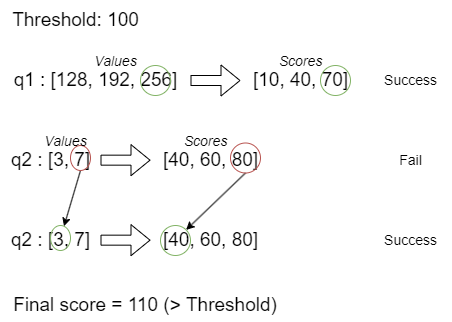
\includegraphics[scale=0.44]{images/Threshold_example.png}}
    \caption{Testing phase with threshold example}
    \label{fig:thex}
\end{figure}

However, such an approach may not have a faster execution time than the current state-of-the-art techniques simply because those techniques imply that the execution phase is composed only of pre-defined test executions over well-aimed and known mechanisms. Therefore, the goal of the proposed solution approach is not to have a faster execution time; instead, it is to have a shorter and more automated overall certification process that would also require considerably fewer resources. Furthermore, directly mapping the properties and attributes to the tests that demonstrate them will be crucial to establishing the values of such attributes. In other words, defining a series of tests are important to determine if a given property or attribute is present. However, to do so efficiently, it is still necessary to have a set of device or system information that would allow the framework to filter out tests that are known to fail.


\subsection{Ephemeral Certificate Meaning}
The volatility or ephemerality of this approach comes from the fact that tests must be light and fast, hence, they cannot be in-depth and ensure a long lasting functioning of the system. (todo?)
